% !TEX root = ../thesis.tex
% results of experiments in chapter 4
% @author Tobias Wulf
%

\chapter{Ergebnisse der Erprobungs- und Optimierungsexperimente 0.0.1 26.04.2021}\label{ch:results-exp}


\section{Vergleich der Kovarianzfunktionen}\label{sec:vgl-kfun-res}


\begin{figure}[tbph]
	\centering
	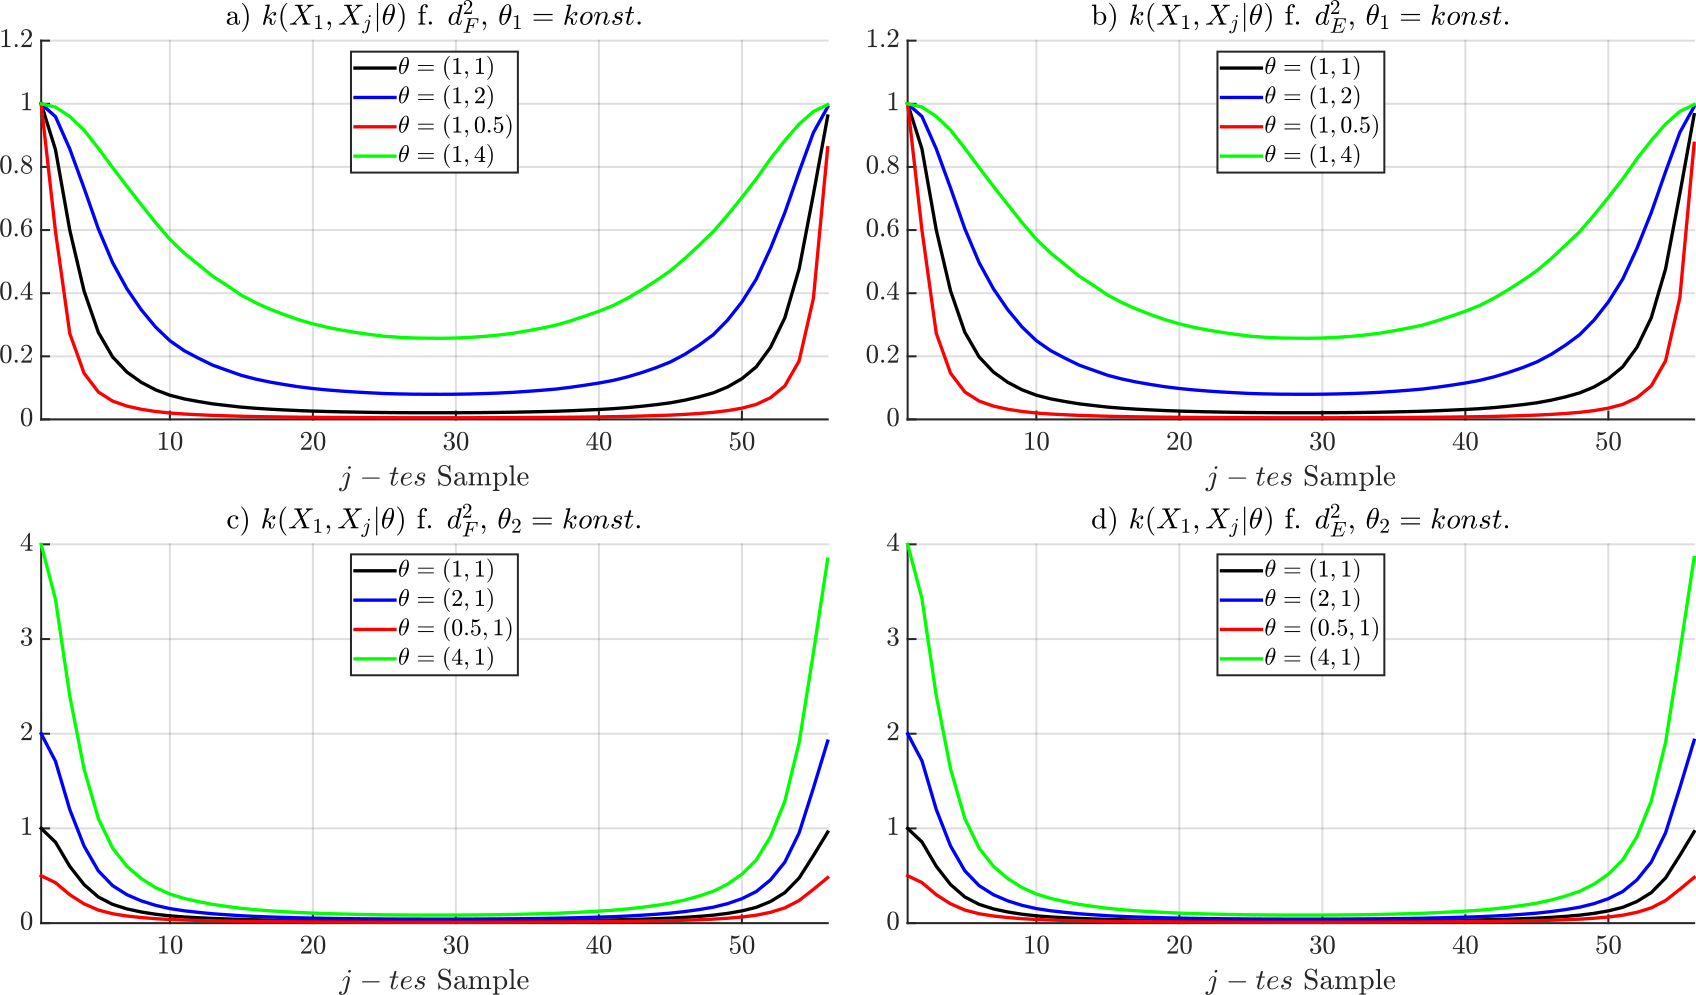
\includegraphics[width=\linewidth]{appendix/images/8-Ergebnisse-Experimente/Vergleich-Kovarianzfunktionen}
	\caption[Kovarianzfunktionen im Vergleich]{Kovarianzfunktionen im Vergleich für variierende Kernel-Parameter $\theta = (\sigma_f^2, \sigma_l)$ und $N=56$ Observerierungen.}
	\label{fig:vergleich-kovarianzfunktionen}
\end{figure}



\begin{figure}[tbph]
	\centering
	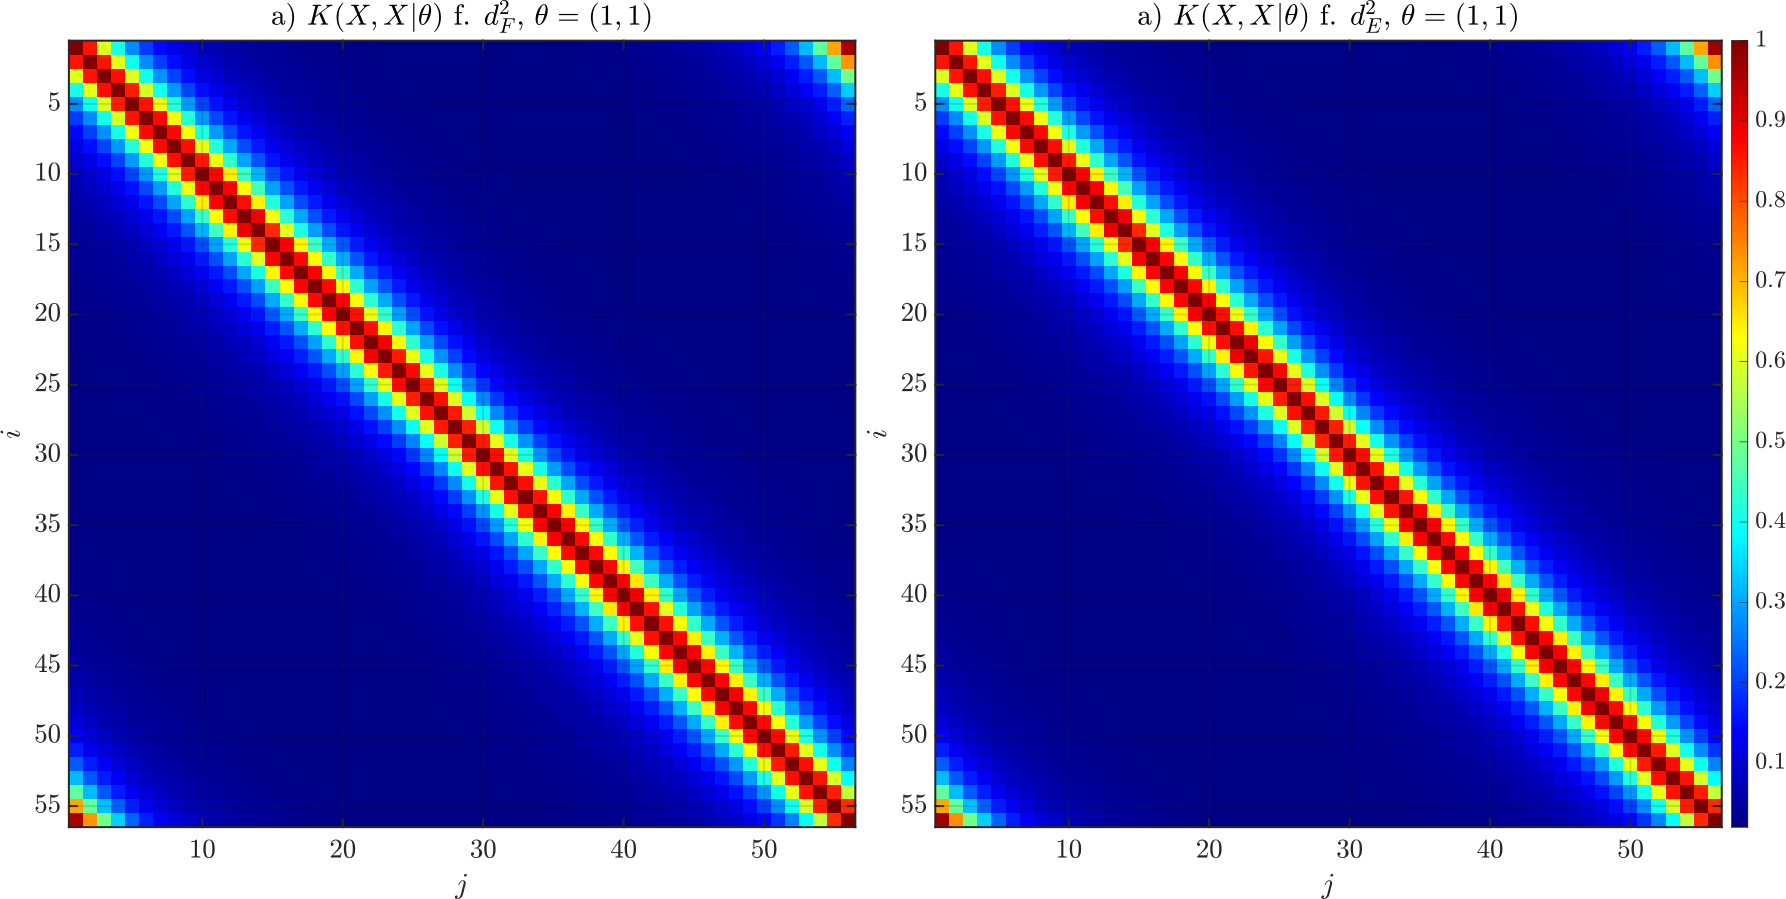
\includegraphics[width=\linewidth]{appendix/images/8-Ergebnisse-Experimente/Vergleich-Kovarianzmatrizen}
	\caption[Gegenüberstellung der Kovarianzmatrizen]{Gegenüberstellung der Kovarianzmatrizen bei ausgeschalter Längen- und und Breitenskalierung mit $\theta = (1,1)$ und $N=56$ Observerierungen.}
	\label{fig:vergleich-kovarianzmatrizen}
\end{figure}


\begin{figure}[tbph]
	\centering
	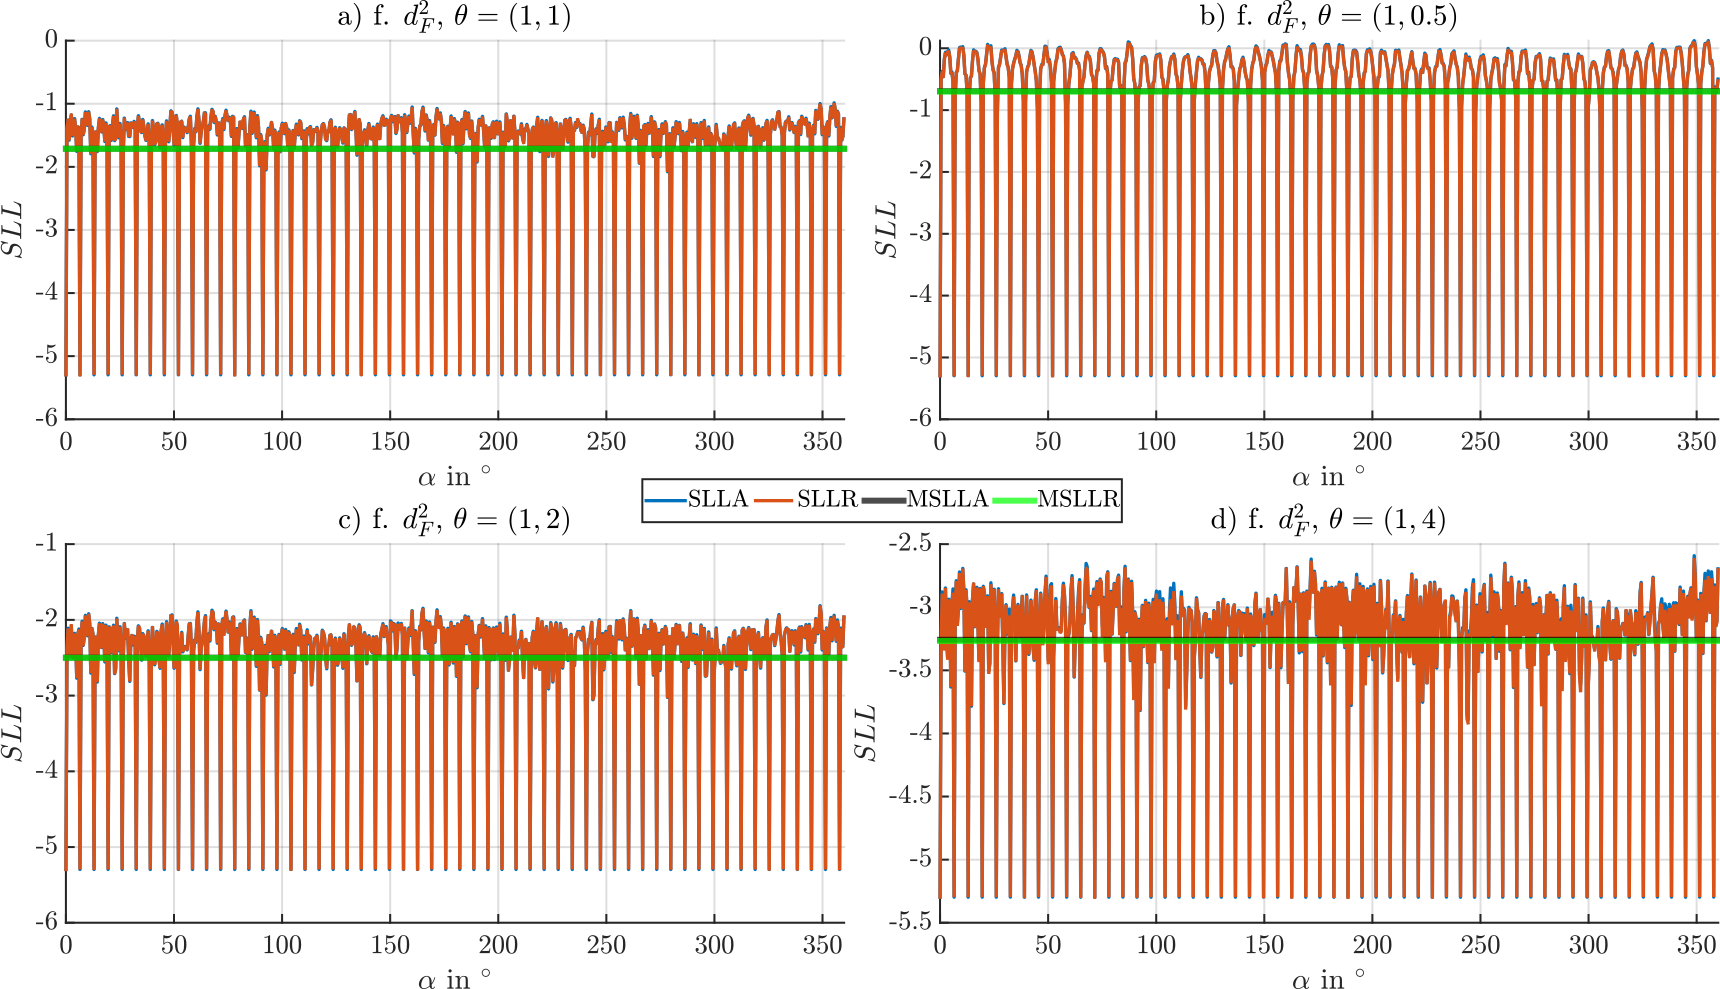
\includegraphics[width=\linewidth]{appendix/images/8-Ergebnisse-Experimente/Vergleich-QFC-SLL}
	\caption[Vergleich der Modellverluste nach Winkel und Radius für die erste Kovarianzfunktion]{Vergleich der Modellverluste nach Winkel und Radius für die erste Kovarianzfunktion für variierende Breitenskalierung.}
	\label{fig:vergleich-qfc-sll}
\end{figure}


\begin{figure}[tbph]
	\centering
	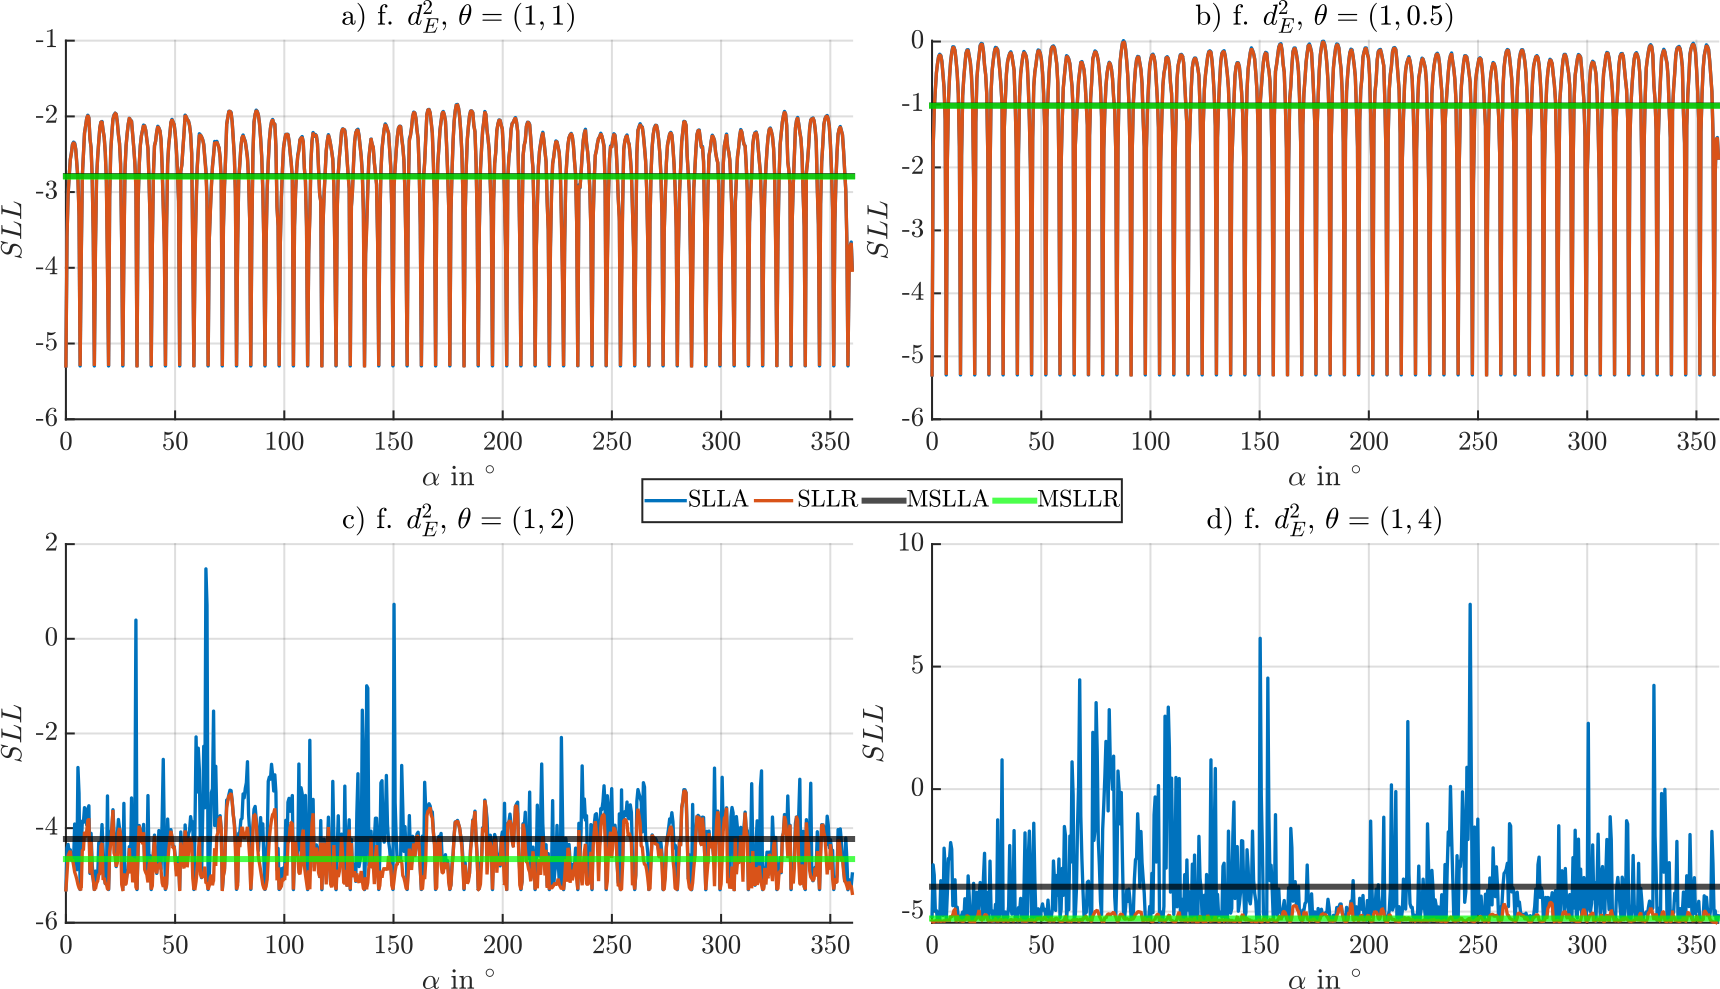
\includegraphics[width=\linewidth]{appendix/images/8-Ergebnisse-Experimente/Vergleich-QFCAPX-SLL}
	\caption[Vergleich der Modellverluste nach Winkel und Radius für die zweite Kovarianzfunktion]{Vergleich der Modellverluste nach Winkel und Radius für die zweite Kovarianzfunktion für variierende Breitenskalierung.}
	\label{fig:vergleich-qfcapx-sll}
\end{figure}

